	\section{EFT description} \label{sec:EFT_Description}

The Higgs potential, before spontaneous symmetry breaking, reads: 

\begin{eqnarray}
  V(\Phi) = - \frac{\mu^2}{2}\left|\Phi \right|^2
  +\frac{\lambda}{4} \left|\Phi \right|^4
  \label{eqm-1}
\end{eqnarray}
where $\Phi$ is the $SU(2)$ doublet scalar field and $\phi = v + H$ is the real part of the neutral component ($v$ being its vacuum expectation value).
The condition of a minimum of the potential leads to the relations:
\begin{eqnarray}
  \lambda = \frac{m_H^2}{2 v^2}, \;\;  \mu^2 = \frac{m_H^2}{2},
  \;\; m_H^2 = \frac{\partial^2 V}{\partial \phi^2}
   \label{eqm-2}
\end{eqnarray}

Therefore, in the SM, the Higgs self-coupling is uniquely determined by the structure of the scalar potential (\ref{eqm-1}), which takes the following
form in terms of the physical $H$ field:

\begin{eqnarray}
  V &=& \frac{m_H^2}{2}H^2 + \lambda_3 v H^3 + \frac{\lambda_4}{4} H^4,
\quad
 \lambda_3 = \lambda_4 = \lambda_{HHH} = \frac{m_H^2}{2v^2} \label{eqm-3}
\end{eqnarray}

However, the sign and value of the parameters $\mu^2$ and $\lambda_{HHH}$ in~(\ref{eqm-1}) are a priori arbitrary.
The positive sign of $\lambda_{HHH}$ is necessary for the stability of the potential at large $\phi$.
Moreover, the functional form of (\ref{eqm-1}) is not fundamental: The underlying gauge
symmetry only requires the potential to depend on $\left| \Phi \right|^2$, and the quartic form could simply represent the leading terms in
the power expansion of a more complex functional dependence of the potential (see~\cite{Mangano:2019kji} for detailed considerations).
Thus, experimentally measuring $\lambda_{HHH}$ is a crucial test of the electroweak symmetry breaking mechanism.
In particular, modifications of the Higgs trilinear couplings (e.g. via a modified Higgs self interaction) can only be directly observed in Higgs boson pair production.

We use the following effective Lagrangian~\cite{deFlorian:2016spz, Carvalho:2015ttv} to describe Higgs boson pair production:

\begin{eqnarray*}\label{Eq:LagrangianBSM}
&&  \mathcal{L}_{BSM} = -{\textcolor{ForestGreen}{\kappa_{\lambda}}} \lambda^{SM}_{HHH} v H^3 -
  \frac{m_t}{v}({\textcolor{blue}{\kappa_t}} H + \frac{\textcolor{red}{c_2}}{v} H^2)(\bar{t_L}t_R + h.c.)
  +  \frac{\alpha_S}{12 \pi v}(\textcolor{red}{c_g} H
  - \frac{\textcolor{red}{c_{2g}}}{2 v}H^2)G^a_{\mu \nu}G^{a, \, \mu \nu} \\
  && {\textcolor{ForestGreen}{\kappa_{\lambda}}} = \frac{\lambda_{HHH}}{\lambda_{HHH}^{SM}}, \;
  \lambda_{HHH}^{SM} = \frac{ m^2_{H}}{2v^2}, \;\;
  {\textcolor{blue}{\kappa_{t}}} = \frac{ y_{t}}{y_{t}^{SM}}, \;\;
  y_{t}^{SM} = \frac{\sqrt{2} m^2_{t}}{ v}
\end{eqnarray*}

\begin{figure}[!htbp]
  \subfloat[SM-like processes]{%
  \label{SMLO_ggHH_production}
            \begin{minipage}[t]{\linewidth}
                  \begin{center}
                          \raisebox{-0.7\height}{ 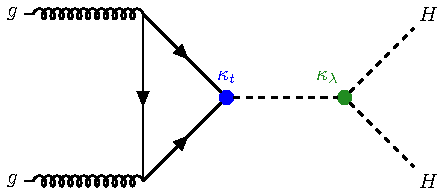
\includegraphics[width=0.45\textwidth]{Images/EFT_Description/fey_HH_Triangle.pdf} }
                          \raisebox{-0.625\height}{ 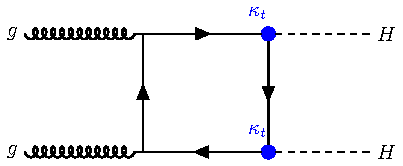
\includegraphics[width=0.45\textwidth]{Images/EFT_Description/fey_HH_Box.pdf} }
                  \end{center} 
          \end{minipage}%
  }
  
  \subfloat[Pure BSM processes]{%
  \label{BSMLO_ggHH_production}
          \begin{minipage}[t]{\linewidth}
                  \begin{center}
                          \raisebox{-0.7\height}{ 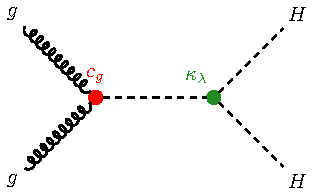
\includegraphics[width=0.30\linewidth,clip]{Images/EFT_Description/fey_HH_anomal_2_colored.pdf} }
                          \raisebox{-0.7\height}{ 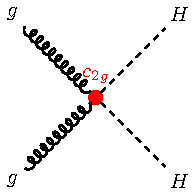
\includegraphics[width=0.20\linewidth,clip]{Images/EFT_Description/fey_HH_anomal_3_colored.pdf} }
                          \raisebox{-0.7\height}{ 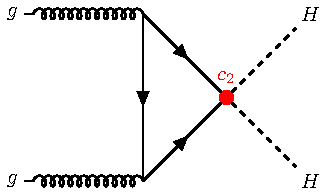
\includegraphics[width=0.30\linewidth,clip]{Images/EFT_Description/fey_HH_anomal_4_colored.pdf} }
                  \end{center}
          \end{minipage}
  }
  \caption{Feynman diagrams for leading-order Higgs boson pair production via gluon fusion}
  \label{fig:ggHH_production}
  \end{figure}
  

where variables are defined as follows:

\begin{itemize} \label{EFT_parameters_description}
  \item $G^a_{\mu \nu} = \partial_{\mu} G_{\nu}^a - \partial_{\nu} G_{\mu}^a + f^{abc}  G_{\mu}^b G_{\nu}^c$ is the gluon field strength tensor
  \item $f^{abc}$ is the totally anti-symmetric $SU(3)$ structure tensor
  \item \textcolor{ForestGreen}{$\kappa_{\lambda}$} - measure of the deviation of the Higgs boson trilinear coupling from its SM expectation $\lambda_{HHH}^{SM}$
  \item \textcolor{blue}{$\kappa_{t}$} - measure of the deviation of the coupling a single Higgs boson and two top quarks from its SM expectation $y_{t}^{SM}$
  \item \textcolor{red}{$c_{2}$} - coupling between two Higgs bosons and two top quarks
  \item \textcolor{red}{$c_{g}$} - coupling between one Higgs bosons and two gluons
  \item \textcolor{red}{$c_{2g}$} - coupling between two Higgs bosons and two gluons
\end{itemize}

The differential cross section of gluon-gluon fusion
induced Higgs boson pair production $\sigma_{HH}$ can be expressed as a polynomial in terms of the
EFT model parameters using generator-level information on the HH system like:

\begin{equation}
\label{eq:rew_3}
  \frac{d^2\sigma}{d m_{HH}d|\cos{\theta^*}| } = \sum A_i( m_{HH}, |\cos{\theta^*}| ) \, c_i
\end{equation}

where the $c_i$ stand for the combinations of couplings as in \cite{Buchalla:2018yce} and $A_i( m_{HH}, |\cos{\theta^*}| )$ are known coefficients.
Eq. (\ref{eq:rew_3}) is used to obtain MC samples corresponding to benchmark samples using a reweighting method \cite{Carvalho:2016rys,Buchalla:2018yce},
where the twenty benchmark scenarios considered in the analysis are shown in Tab. \ref{tab:eft_bench} \cite{Carvalho:2015ttv,Buchalla:2018yce,Capozi:2019xsi}. 

The $\kappa_{\lambda}$ parameter also affects the Higgs boson branching ratios and the single Higgs production cross sections because of next-to-leading (NLO) electroweak corrections \cite{Degrassi:2016wml,Maltoni:2017ims}.

\begin{table}[h]
  \begin{center}
    \begin{tabular}{r|ccccc}
      Benchmark & $\kappa_{\lambda}$ & $\kappa_{t}$ & $c_{2}$	& $c_{g}$ & $c_{2g}$ \\ \hline
      SM &	1.0 & 1.0	 &	0.0		& 0.0	& 0.0 \\ \hline
      1 &	7.5	 & 1.0	 &	-1.0	& 0.0	& 0.0 \\
      2 &	1.0	 & 1.0	 &	0.5		& -0.8	& 0.6 \\
      3 &	1.0	 & 1.0	 &	-1.5	& 0.0	& -0.8 \\
      4 &	-3.5 & 1.5  &	-3.0	& 0.0	& 0.0 \\
      5 &	1.0	 & 1.0	 &	0.0		& 0.8	& -1 \\
      6 &	2.4	 & 1.0	 &	0.0		& 0.2	& -0.2 \\
      7 &	5.0	 & 1.0	 &	0.0		& 0.2	& -0.2 \\
      8 &	15.0 & 1.0	 &	0.0		& -1	& 1 \\
      9 &	1.0	 & 1.0	 &	1.0		& -0.6	& 0.6 \\
      10 &	10.0 & 1.5   &	-1.0	& 0.0	& 0.0 \\
      11 &	2.4	 & 1.0	 &	0.0		& 1		& -1 \\
      12 &	15.0 & 1.0	 &	1.0		& 0.0	& 0.0 \\[0.5ex] \hline 
      8a &  1.0  & 1.0   &  0.5   & $\frac{0.8}{3}$ & 0.0 \\[0.5ex] 
      1b &  3.94 & 0.94  & $\frac{-1}{3}$ & 0.75 & -1 \\[0.5ex] 
      2b &   6.84 & 0.61 &  $\frac{1}{3}$ &  0.0 & 1.0 \\[0.5ex] 
      3b &   2.21 & 1.05 & $\frac{-1}{3}$ &  0.75 &  -1.5 \\[0.5ex] 
      4b &   2.79 & 0.61 &  $\frac{1}{3}$ & -0.75 &  -0.5 \\[0.5ex] 
      5b &   3.95 & 1.17 & $\frac{-1}{3}$ & 0.25 &  1.5 \\[0.5ex] 
      6b &   5.68 & 0.83 &  $\frac{1}{3}$ & -0.75 &  -1.0 \\[0.5ex] 
      7b &   -0.10 & 0.94 &         1.0 & 0.25 & 0.5 \\
    \end{tabular}
  \end{center}
  \caption{Parameter values of the 20 EFT benchmarks and the Standard Model. \label{tab:eft_bench}}
\end{table}
